\section{Hands on datasets}
Before looking at the machine learning algorithms, let us focus on how to prepare data to be fed to the algorithms. The focus is on the \textit{scikit-learn} and \textit{Pandas} libraries in Python and .

\subsection{Looking at data}
After having loaded the data in a Pandas dataframe, there are methods of this data structure that allow to get some information from the data:
\begin{itemize}
\item \textbf{\textit{df.head()}}: this method allows to get a gist on the general structure of the dataframe by looking at the value of the first 5 rows. More rows can be shown by passing as input the desired number to be shown;

\item \textbf{\textit{df.info()}}: it tells the number of entries and for each column its type and the number of non-null elements. Note that string type is considered in a more general type as \textit{object} type;
\item \textbf{\textit{df['field'].value\_counts()}}: this is useful when \textit{field} is a categorical. It shows all the possible values in the dataframe for the column and for each one the number of entries having that column value;
\item \textbf{\textit{df.describe()}}: this method performs some statistics on numerical attributes (null values are ignored). Particularly, it calculates the number of entries (with valid values), the mean, standard deviation, minimum and maximum and the $25\%, 50\%, 75\%$ percentiles.
\item\textbf{\textit{df.hist(bins=20)}}: it plots the histogram of each numerical value. The number of bins tells how many bars (i.e., how many groups) the histogram should have;
\item\textbf{\textit{df.corr()['attribute'].sort\_values(ascending=False)}}: shows the correlation between the selected attribute and all the others. Remember that the correlation an indication of linear relationships only;
\item\textbf{\textit{scatter\_matrix(h[attributes], figsize=(12,8))}}: plots every numerical attribute against every other numerical attribute (carefulness is needed when the number of attribute is large). To give some sense to the main-diagonal plots, a histogram is plotted by the function itself. See \autoref{scatterplot}.
\end{itemize}

Some inferences can be made from the histogram. First of all the units and scales; there even might be some hints if values have been cupped (for example when there is a natural decreasing trend but the last bin has a value significantly bigger than the others).

\subsection{Train and test set}
The first thing to do is to split the set between train and test. A good idea is to have the same split across different runs of the algorithms. One solution is to save the data-set and load it next times. Another solution is to use random generator seeds so that the pseudo-random sequence starts every-time from the same point. But these solutions will break next time one fetches an updated dataset. 

A common solution is to use each instance's identifier to decide whether or not it should go in the test set (assuming instances have a unique and immutable identifier). For example, you could compute a hash of each instance's identifier, keep only the last byte of the hash, and put the instance in the test set if this value is lower or equal to 51 (~20\% of 256). This ensures that the test set will remain consistent across multiple runs, even if you refresh the dataset. It is assuming a uniform distribution by hash algorithm. This can be implemented with the following functions:

\begin{lstlisting}[caption=Example of function to split according to the last by of the hash on the id.]
def split_train_test_by_id(data, test_ratio, id_column, 
		                        hash=hashlib.md5):
    ids = data[id_column];
    in_test_set = ids.apply(lambda _id: test_set_check(_id,  test_ratio, hash));
    return data.loc[~in_test_set], data.loc[in_test_set];

# The check on the id is to see the value of the last byte
# If this value is less then test_ratio*256 (assuming uniform 
# distribution) 
# then will return true otherwise false. The fraction of true
# will be  equal to test_ratio
def test_set_check(identifier, test_ratio, hash):
    limit = test_ratio*256; #1byte
     #digest will calculate the hash value 
    res = hash(np.int64(identifier)).digest()[-1];
    return res<limit;
\end{lstlisting}

However, there is a \tb{further problem} if there is not an identifier column. The solution is to create one. It is possible to use the row index but the one has make sure new data are appended in order and no data should not be deleted.If this is not possible, then you can try to use the most stable features to build a unique identifier. For example, a district's latitude and longitude are guaranteed to be stable for a few million years, so one could combine them into an ID like so and their values are unique:
\begin{lstlisting}[caption="Creating a column ID from stable features such as latitude and longitude.]
df["id"] = df['longitude']*1000+df['latitude']
\end{lstlisting}

\subsubsection{Stratified sampling}
Consider a given value, either categorical or numerical. Generally, they are not uniformly distributed among the entries. As the simplest possible example consider that in a data set of people women are the $60\%$, and men $40\%$. When splitting between train and test set it is better to keep this ratio, especially when some values are rarer.

This is true also for numerical value: in this case, one first needs to create a corresponding categorical attribute. It is important to have sufficient data for each category and at the same time categories must be representatives. First a range size is chosen (the range of the new categorical value) and it is used to divide the original values. Then the resulting valued are ceiled. Clapping is required.

After that, it is possible to stratify-sampling. \ti{scikit-learn} has the function \ti{StratifiedShuffleSplit} to perform it:
\begin{lstlisting}
from sklearn.model_selection import StratifiedShuffleSplit
split = StratifiedShuffleSplit(n_splits=1, test_size=0.2, random_state=42);
\end{lstlisting}

\subsection{Plotting the dataset}
Visualing data can give other insights.
Pandas dataframe has a plot method:
\begin{lstlisting}[caption=Example of Pandas dataframe plot method.]
df.plot(kind="scatter", x="longitude", y="latitude", alpha=0.2);
\end{lstlisting}
In this way one gets darker areas according to the number of elements.
It is also to make more complex graphs: for example we can use colormaps to represent the intensity of output and circle radius to represent another feature of the data:
\begin{lstlisting}[caption=Example of Pandas dataframe plot with colormap and variable radius of scattered circles.]
h.plot(kind="scatter",x="longitude", y="latitude", alpha=0.4, 
		s = h['population']/100,  label="popultion", 
		c="median_house_value", cmap = plt.get_cmap('jet'), 
		colorbar=True, figsize=(15,8));
plt.legend();
\end{lstlisting}

\begin{figure}
\centering
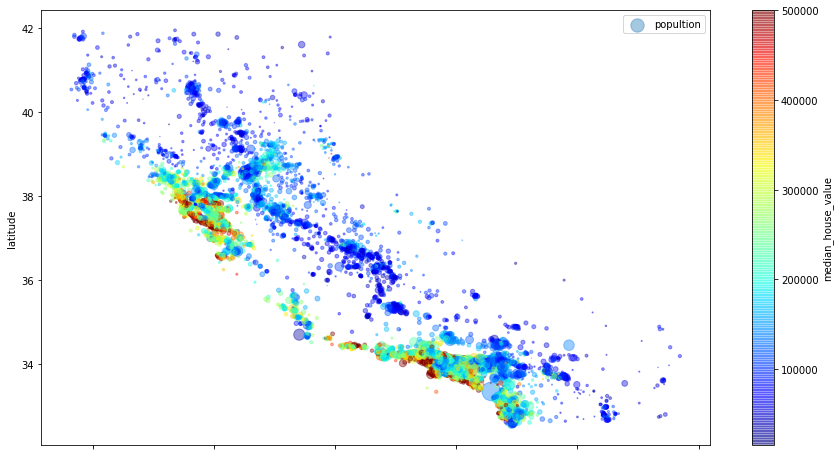
\includegraphics[scale=0.45]{img/DatasetCmap}
\caption{Example of plotting a dataframe. The latitude is plotted over the longitude. The color tells the intensity of the output variable while the circle radius tells are related to another input variable (population).}
\label{californiaHouses}
\end{figure}

\autoref{californiaHouses} shows the prices of Californian houses using a colormap in terms of geographical position and population.
This image tells you that the housing prices are very much related to the location (e.g., close to the ocean) and to the population density, as you probably knew already. It will probably be useful to use a clustering algorithm to detect the main clusters, and add new features that measure the proximity to the cluster centres. 

\subsection{Interpretation of scatter plot}
\label{scatterplot}
This method is important: it gives an idea of which variable are related: if the graph looks uniform then maybe there is no relation. On the contrary other, other patterns might be visible. For example, from \autoref{scatter_img} it is possible to see a strong correlation between \ti{median\_house\_value} and \ti{median\_income}.
\begin{figure}
\centering
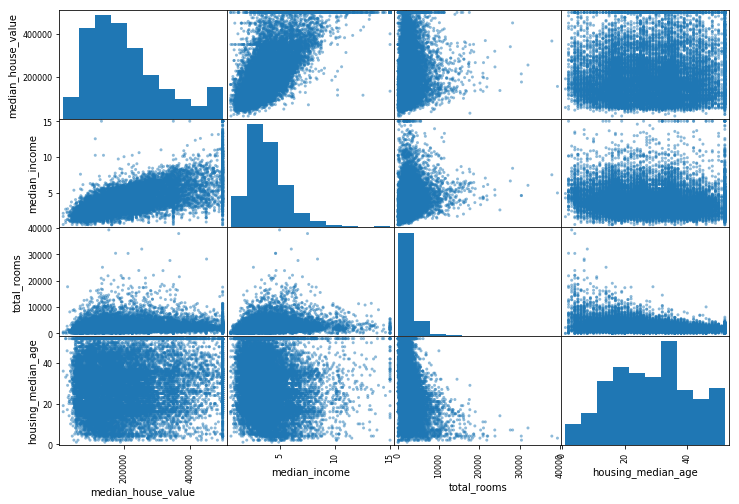
\includegraphics[scale=0.51]{img/scatterplot}
\caption{Example of scatterplot for some attributes of the California houses dataset.}
\label{scatter_img}
\end{figure}

Looking closer at it in \autoref{singleScatterPlot},
\begin{figure}
\centering
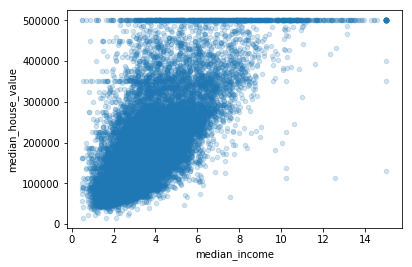
\includegraphics[scale=0.8]{img/singleScatterPlot}
\caption{Scatterplot of the attributes \ti{median\_house\_value} and \ti{median\_income}.}
\label{singleScatterPlot}
\end{figure}

\autoref{singleScatterPlot} shows these two variables are really correlated. We also notice the horizontal line at $\$500,000$ since data prices are capped.

However, there are other horizontal lines at $\$450,000$, at $\$380,000$ and maybe one at $\$280,000$. Maybe it is better to remove these districts so that the algorithm does not learn to reproduce them.

\subsection{Data manipulation}
Some values need to be properly interpreted. In the California houses data set the attribute \ti{total\_bedrooms} is the total number of rooms in a district. Rather than that, it is better to consider the approximated number of bedrooms per house, obtained by dividing the former by the total number of houses in that district. This new attribute will be more correlated to the output than the original one. Apparently houses with a lower bedroom/room ratio tend to be more expensive. 
In the same way, the number of rooms per household is also more informative than the total number of rooms in a district - obviously the larger the houses, the more expensive they are.

\subsubsection{Convert categorical values to numerical values}
Many machine algorithms work with numerical attributes and not with categorical values. It is a good idea to convert these categorical value to a numerical value. \ti{SciKit-learn} offers the \ti{LabelEncoder} class, which convert each categorical value to a number:
\begin{lstlisting}[caption=Example of usage of \ti{LabelEncoder} class]
from sklearn.preprocessing import LabelEncoder
encoder = LableEncoder();
encoder = LabelEncoder();
h_cat = h['ocean_proximity'];
h_cat_encoded = encoder.fit_transform(h_cat);
\end{lstlisting}
where \ti{ocean\_proximity} is a categorical attribute. However, there is a problem with this representation:  ML algorithms will assume that two nearby values are more similar than two distant values. Many times this is not guaranteed to be the case. To fix this issue, a common solution is to create one binary attribute for each possible categorical value. This is called \tb{one-hot encoding}, because only one attribute will be equal to 1 (hot), while the others will be 0 (cold).

\ti{SciKit-learn} provides \ti{OneHotEncoder} to convert integer categorical value into one-hot vectors. This function seems to be deprecated though.

\begin{lstlisting}[caption=Usage of \ti{ColumnTransformer}]
from sklearn.compose import ColumnTransformer
h_copy = h.copy()
ct = ColumnTransformer([("onehot",OneHotEncoder(),[h_copy.columns.get_loc('ocean_proximity')])]);
onehot = ct.fit_transform(h_copy.values).astype('int').toarray();
onehot
Out:
array([[1, 0, 0, 0, 0],
       [1, 0, 0, 0, 0],
       [0, 0, 0, 0, 1],
       ...,
       [0, 1, 0, 0, 0],
       [1, 0, 0, 0, 0],
       [0, 0, 0, 1, 0]])
\end{lstlisting}
Apparently \ti{ColumnTransformer} has no inverse so we are loosing the references to the category
We create a dataframe containing the encoding of the categorical variables and then we merge it to the original dataframe:
\begin{lstlisting}[caption=Usage of \ti{LabelBinarizer}]
from sklearn.preprocessing import LabelBinarizer
# sparse_output=True compresses the matrix not to use too much mem, 
# toarray() allows to get back the array
h_copy = h.copy();
enc = LabelBinarizer(sparse_output=True);
onehot = enc.fit_transform(h_copy['ocean_proximity']);
enc.inverse_transform(np.identity(onehot.shape[1])).reshape(-1,);
ocean_prox_df = pd.DataFrame(
		data=onehot.toarray().astype('int'), 
		columns=enc.inverse_transform(np.identity(onehot.shape[1])));

# Now we concatenate the original and one-hot encoded datafram
h_cat = pd.concat([h_copy.drop('ocean_proximity', axis=1), 
		ocean_prox_df], axis=1);
h_cat
\end{lstlisting}

Alternatively, Pandas dataframe data structure has its own simpler method \ti{pandas.get\_dummies(df.categorical\_attribute}:
\begin{lstlisting}[caption=Usage of \ti{pd.get\_dummies()}]
h_copy = h.copy();
ocean_prox_dummies = pd.get_dummies(h_copy.ocean_proximity);
h_res = pd.concat([h_copy, ocean_prox_dummies], axis=1);
h_res.drop('ocean_proximity', axis=1, inplace=True);
\end{lstlisting}

\subsection{Data cleaning}
One big problem are missing values. These can be replaced with different techniques:
\begin{itemize}
\item \tb{\ti{df.dropna(subset=["total\_bedrooms"]);}}: gets rid of the entries having null for this column(s);
\item \tb{\ti{df.drop("total\_bedrooms", axis=1);}}: gets rid of the entire attribute;
\item \tb{\ti{df["total\_bedrooms].fillna(median);}}: set the missing value to the specified value (0, mean, median).The value (\ti{median} in this case) has been computed with the training set so it must be saved
\end{itemize}

If more than one column has missing values, we can use the SciKitLearn class \ti{Imputer}. Its constructor takes as input a string parameter called \ti{strategy} that specifies the value replacement. An example is the following:
\begin{lstlisting}[caption=Usage of \ti{SimpleImputer to clean data}]
from sklearn.preprocessng import SimpleImputer
imputer = SimpleImputer(strategy="median");
h_num = h.drop('ocean_proximity', axis=1);
imputer.fit(h_num);
imputer.statistics_;
X = imputer.transform(h_num); #output is a numpy array
h_tr = pd.DataFrame(X, columns =h_num.columns)
\end{lstlisting}

\subsection{Custom Transformers}
\ti{Scikit} allows you to create your own transformers using \tb{ducking type programming style}. In ducking type, an object passed into a function must support all methods and attributes it s expected to have at runtime. The object type itself does not matter: in this sense, it is very different from inheritance. 

For \ti{Transformers}, three methods must be implemented:
\begin{itemize}
\item\ti{fit();}: this method just calculates the parameter and it is run on the training set. The parameters are saved as internal object state.
\item \ti{transform();}: it applies the transformation to a particular set of examples. it can be called right after \ti{fit()} on the training set or on the test set (on which one does not call \ti{fit})
\item \ti{fit\_transform();}: joins these two steps and is used for the initial fitting of parameters on the training set, but it also returns a transformed set. Internally, it just calls first \ti{fit()} and then \ti{transform()} on the same data.
\end{itemize}
We can get the last one for free exploiting inheritance from the base class \ti{\tb{TransformerMixin}}. By adding also \ti{\tb{BaseEstimator}} as a base class and avoiding \ti\tb{*args} and \ti\tb{*kargs} in the constructor, we will get the extra methods \ti\tb{get\_params} and ti\tb{set\_params} that will be useful for automatic hyperparameter tuning.

\begin{lstlisting}[caption=Example of how to create a custom transformer.]
from sklearn.base import BaseEstimator, TransformerMixin

rooms_ix, bedrooms_ix, population_ix, household_ix = 3, 4, 5, 6;

class CombinedAttributesAdder(BaseEstimator, TransformerMixin):
    def __init__(self, add_bedrooms_per_room=True):
        self.add_bedrooms_per_room = add_bedrooms_per_room;

    def fit(self, X, y=None):
        return self;
    
    def transform(self, X, y=None):
        rooms_per_household = X[:,rooms_ix]/X[:, household_ix];
        population_per_household = X[:,population_ix]/X[:, household_ix];
        if self.add_bedrooms_per_room:
            bedrooms_per_room = X[:,bedrooms_ix]/X[:, rooms_ix];
            return np.c_[X, rooms_per_household, population_per_household, bedrooms_per_room];
        else:
            return np.c_[X, rooms_per_household, population_per_household];
        
attr_adder = CombinedAttributesAdder(add_bedrooms_per_room=False);
h_extra_attribs= attr_adder.transform(h_copy.values);
\end{lstlisting}

\subsection{Feature scaling}
In general, inputs have very different scales. ML algorithms work better if inputs have the same scale. For this reason, they are scaled before applying the algorithm. Tow popular scaling methods are the following:
\begin{itemize}
\item \ti{\tb{min-max}} or \ti{\tb{normalization}}: values are scaled to be in range $[0,1]$. Minimum value is subtracted and then it is scaled by the maximum value. \ti{Scikit} provides \ti{MinMaxScaler} with \ti{feature\_range} property to change the range.
\item \ti{\tb{standardization}}: it subtracts the mean value (0-mean) and then divides by the variance to have a unit variance distribution. Standardization is much less affected by outliers but might be a problem for some algorithms (such as NN) expecting values to be within a given range.
\end{itemize}

\subsection{Scikit-learn transformation pipeline}
The \ti{pipeline} data structure allows to collect the transformation to be applied to the dataset. All but last estimator must be transformers, i.e., they must have the method \ti{fit\_transform}. When one calls the pipeline's \ti{fit()}method, it calls \ti{fit\_transform()} sequentially on all transformers, passing the output of each call as the parameter to the next call, until it reaches the final estimator, for which it just calls the \ti{fit()} method and then \ti{transform()}.
\begin{lstlisting}
from sklearn.pipeline import Pipeline
from sklearn.preprocessing import StandardScaler
from sklearn.impute import SimpleImputer
num_pipeline = Pipeline([('imputer', SimpleImputer(strategy='median')),
                        ('attribs_adder', CombinedAttributesAdder()),
                         ('std_scaler', StandardScaler())
                        ]);
h_num_tr = num_pipeline.fit_transform(h.drop('ocean_proximity',axis=1));
\end{lstlisting}
\subsubsection{Perform parallel transformations}
The scaling of numerical values and the transformation of categorical values to many binary attributes are independent, hence they can be performed in parallel.

Scikit provides \ti{\tb{FeatureUnion}} class. You give it a list of transformers (which can be entire transformer pipelines), and when its \ti{\tb{transform()}} method is called, it runs each transformer’s \ti{\tb{transform()}} method in parallel, waits for their output, and then concatenates them and returns the result (and of course calling its \ti{\tb{fit()}} method calls all each transformer’s \ti{\tb{fit()}} method). 

Before looking at the \ti{FutureUnion}, we needed two more pieces. First of all, each subpipeline starts with a selector transformer: it simply transforms the data by selecting the desired attributes (numerical or categorical), dropping the rest, and converting the resulting DataFrame to a NumPy array. There is nothing in Scikit-Learn to handle Pandas DataFrames, so we need to write a simple custom transformer for this task. The code in \autoref{SelectorTransfomer} does this.

\begin{lstlisting}[
caption=Transformer to select the desired attributes of a Pandas dataframe,
 label=SelectorTransfomer]
from sklearn.base import BaseEstimator, TransformerMixin

class DataFrameSelector(BaseEstimator, TransformerMixin):
    def __init__(self, attribute_names):
        self.attribute_names = attribute_names;
    def fit(self, X, y=None):
        return self;
    def transform(self, X):
        return X[self.attribute_names].values
\end{lstlisting}

Secondly, the method \ti{fit\_transform()} of \ti{LabelBinarizer} changed from SciKit-learn version 0.18 to 0.19. The problem is that now it accepts just two inputs: the instance and the array to be encoded: \ti{lb.fit\_transform(['yes', 'no', 'no', 'yes'])}, while the pipeline requires three.
We create a new class \ti{LabelBinarizerPipelineFriendly} which inherits from \ti{LabelBinarizery} overload \ti{fit\_transform()} method to accept another parameter \ti{y} that actually it is not used. The method first calls \ti{fit} and then \ti{transform()}. See \autoref{LabelBinarizerPipelineFriendly}.
\begin{lstlisting}[
caption=Custom LabelBinarizer class that can be used in a pipeline, 
label=LabelBinarizerPipelineFriendly]
class LabelBinarizerPipelineFriendly(LabelBinarizer):
     def fit(self, X, y=None):
         """this would allow us to fit the model based on the X input."""
         super(LabelBinarizerPipelineFriendly, self).fit(X)
     def transform(self, X, y=None):
         return super(LabelBinarizerPipelineFriendly, self).transform(X)

     def fit_transform(self, X, y=None):
         return super(LabelBinarizerPipelineFriendly, self).fit(X).transform(X)
\end{lstlisting}

Finally we can use \ti{FutureUnion} as in \autoref{FutureUnion}.
\begin{lstlisting}[caption=Usage of \ti{FutureUnion}, label=FutureUnion]
from sklearn.pipeline import FeatureUnion;
num_attr = list(h.drop('ocean_proximity',axis=1))
cat_attr = ['ocean_proximity']
num_pipeline = Pipeline([
                        ('selector', DataFrameSelector(num_attr)),
                        ('imputer', SimpleImputer(strategy='median')),
                        ('attribs_adder', CombinedAttributesAdder()),
                        ('std_scaler', StandardScaler())
                        ]);
cat_pipeline = Pipeline([
                        ('selector'       , DataFrameSelector(cat_attr)),
                        ('label_binarizer', LabelBinarizerPipelineFriendly())#using custom because fit_transform method changed
                        ]);
full_pipeline = FeatureUnion(
            transformer_list =[
                              ("num_pipeline", num_pipeline), 
                              ("cat_pipeline", cat_pipeline)
                              ]);
h_prepared = full_pipeline.fit_transform(h);
\end{lstlisting}